\chapter{Deseño do software}
Neste capítulo descríbese a arquitectura do sistema a desenvolver desde un punto de vista global, identificando as distintas compoñentes que o conforman e a forma de relacionarse entre elas, tanto dende o punto de vista estrutural como de interacción entre elas.

\section{Arquitectura do sistema}
Dende a definición dos obxectivos do proxecto identifícanse dúas partes diferenciadas dentro do sistema a desenvolver. Por un lado a comunicación co servidor SOS, para a obtención das súas capacidades e dos datos de observacións, e por outro a visualización e explotación das observacións descargadas. Esta división trasladase directamente á estrutura da aplicación, que se amosa na figura \ref{fig:diaComponentes}. Tamén se inclúen os compoñentes externos cos que se relacionan.

\begin{figure}[hbtp]
 \centering
 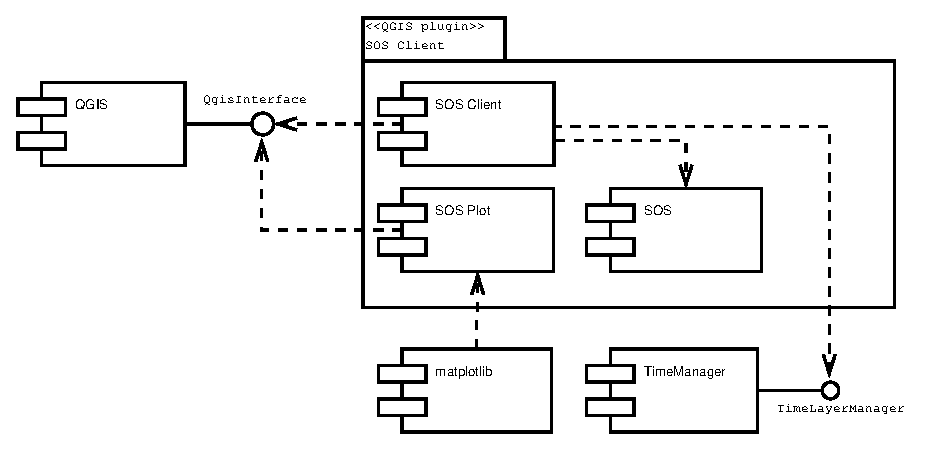
\includegraphics[width=0.5\textwidth]{images/componentes.eps}
 \caption{Diagrama de compoñentes}
 \label{fig:diaComponentes}
\end{figure}

A compoñente \textbf{SOS Client} é a responsable da comunicación co servidor SOS tanto á hora de xerar as peticións necesarias a partir da información proporcionada polo usuario, como para almacenar e interpretar as respostas do servizo.

A compoñente \textbf{SOS Plot} é a responsable de, a partir da capa vectorial xerada, visualizar as observacións segundo as preferencias indicadas polo usuario.

As compoñentes externas incluídas no diagrama son:
\begin{itemize}
\item QGIS: Representa á aplicación na que se integra o \emph{plugin}.
\item TimeManager\footnote{\url{https://plugins.qgis.org/plugins/timemanager/}}: É un \emph{plugin} para QGIS que engade controles de tempo ó mesmo, de xeito que se podan animar as capas vectoriais directamente no visor de mapas, en base a un atributo de tempo.
\item matplotlib\footnote{\url{http://matplotlib.org/}}: É unha librería de Python para debuxar gráficos en 2D que permite producir figuras de alta calidade, tanto para publicacións como en entornos interactivos.
\end{itemize}

\subsection{Patrón de arquitectura}
O uso dun patrón de arquitectura axeitado para o sistema a desenvolver facilita os procesos de implementación e probas, ó proporcionar un esquema de organización estrutural dividindo o sistema en partes segundo a súa responsabilidade.

Os patróns de arquitectura máis amplamente utilizados no desenvolvemento de aplicacións son o MVC (\emph{Model-View-Controller}) e os seus derivados. O obxectivo principal destes patróns é separar o modelo de datos, a súa visualización e a lóxica de negocio facilitando de xeito moi significativo o mantemento e evolución das aplicacións.

Dadas as características concretas desde desenvolvemento optouse por unha simplificación do patrón MVC combinando a lóxica de negocio coas vistas, dando lugar a unha arquitectura denominada \emph{Model/View}\footnote{\url{http://doc.qt.io/qt-4.8/model-view-programming.html}}. Os motivos principais para levar a cabo esta simplificación son:
\begin{itemize}
\item A lóxica de negocio da aplicación e moi sinxela.
\item As librerías para o desenvolvemento das vistas veñen impostas pola aplicación na que se integrará o \emph{plugin}. As propias librerías están deseñadas para facilitar este patrón.
\end{itemize}

É importante destacar que aínda que se se incorpore a lóxica de negocio nas vistas, si que se mantén a separación entre a creación e configuración dos compoñentes gráficos do resto de lóxica da vista. A creación dos compoñentes gráficos faise a través dunha factoría que os xera directamente desde a súa definición XML.

Na figura \ref{fig:MVCvsMV} móstrase de xeito gráfico a diferencia entre o patrón MVC e o \emph{Model/View}. O \emph{Model/View}, amais da vista e o modelo, inclúe o concepto \emph{Delegate}, que representa a un mediador entre a vista e o modelo para facilitar a personalización de como se mostran e editan determinados datos.

\begin{figure}[hbtp]
 \centering
 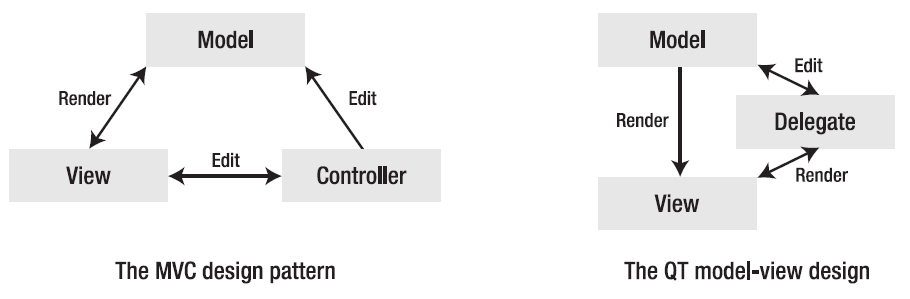
\includegraphics[width=\textwidth]{images/MVCvsMV.png}
 \caption{Diferencias entre MVC e Model/View}
 \label{fig:MVCvsMV}
\end{figure}

\section{Interacción entre compoñentes}
Para describir o comportamento do sistema desde un punto de vista dinámico empréganse os diagramas de secuencia, nos que se describe a interacción entre as distintas compoñentes do sistema para cumprir cada caso de uso definido.

Para conseguir un nivel de detalle suficiente para describir o comportamento do sistema dividisen as compoñentes segundo a arquitectura \emph{Model/View} proposta. A compoñente SOSClient divídese en SOSClientDialog, que representa a vista, e Sensor Observation Service, que representa o modelo. No caso da compoñente SOSPlot, a vista é representada pola compoñente SOSPlotDialog e o modelo non se representa de xeito independente pois está incluído dentro da compoñente matplotlib.

No diagrama \ref{fig:diaSeq1-2} inclúense os caso de uso \ref{uc:CU.01} e \ref{uc:CU.02}, xa que o \ref{uc:CU.02} estende ó \ref{uc:CU.01}, polo que é máis claro representalos xuntos.
\begin{figure}
 \centering
 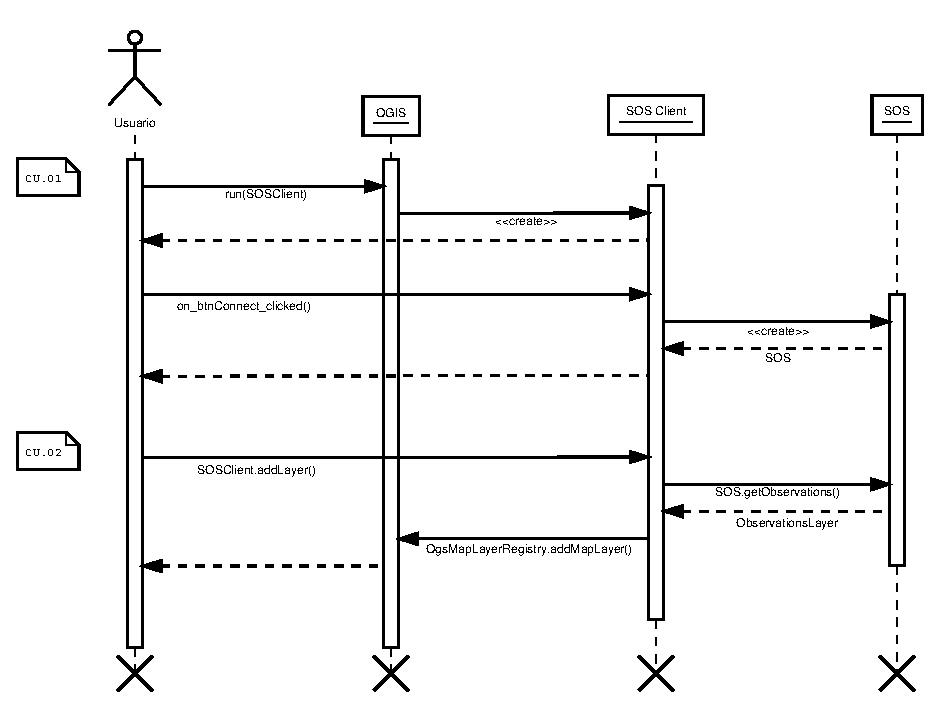
\includegraphics[width=\textwidth]{images/seq1-2.eps}
 \caption{Diagrama de secuencia para os casos de uso \ref{uc:CU.01} e \ref{uc:CU.02}}
 \label{fig:diaSeq1-2}
\end{figure}

O diagrama \ref{fig:diaSeq3} representa o comportamento para o caso de uso \ref{uc:CU.03}.
\begin{figure}
 \centering
 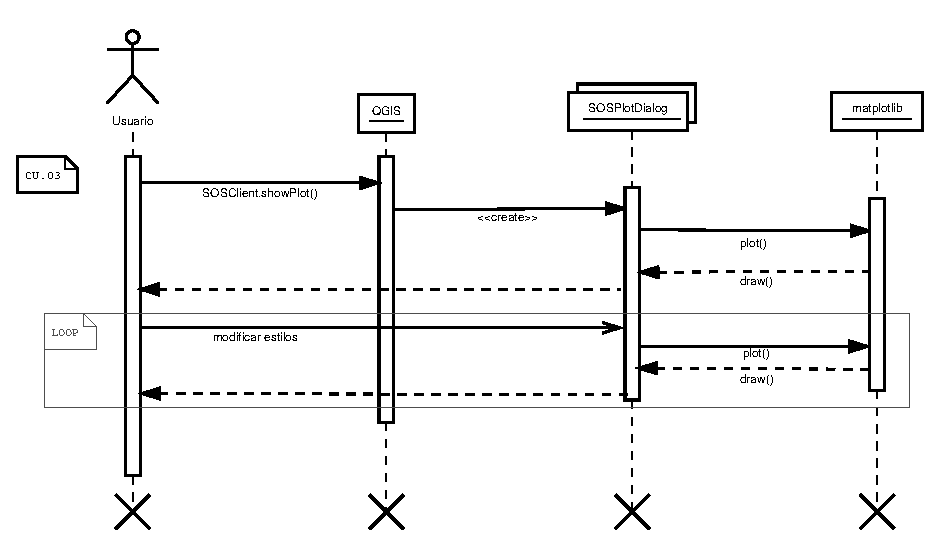
\includegraphics[width=\textwidth]{images/seq3.eps}
 \caption{Diagrama de secuencia para o caso de uso \ref{uc:CU.03}}
 \label{fig:diaSeq3}
\end{figure}

Para cubrir a funcionalidade requirida polo caso de uso \ref{uc:CU.04} existe o \emph{plugin} \emph{TimeManager} para QGIS, polo que o que representa o diagrama \ref{fig:diaSeq4} é o procedemento para que a capa xerada coas observacións sexa controlada polo \emph{TimeManager}.
\begin{figure}
 \centering
 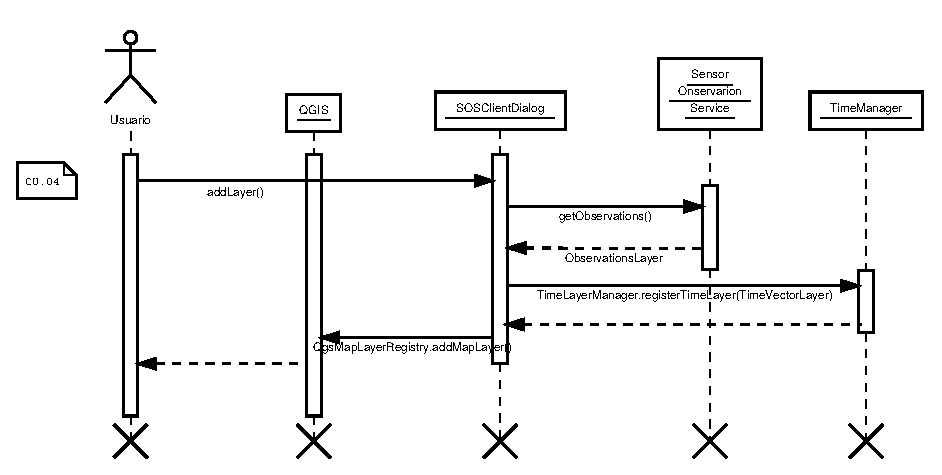
\includegraphics[width=\textwidth]{images/seq4.eps}
 \caption{Diagrama de secuencia para o caso de uso \ref{uc:CU.04}}
 \label{fig:diaSeq4}
\end{figure}